\documentclass[numbers=noenddot,12pt,a4paper]{scrartcl}
\usepackage[greek,ngerman]{babel}
\usepackage[T1]{fontenc}
\usepackage[utf8]{inputenc}
\usepackage{fullpage}
\usepackage{libertine}
\usepackage{ziffer}
\usepackage{graphicx}
\usepackage{units}
\usepackage[infoshow]{tabularx}
\usepackage{amsmath}
\usepackage{amssymb}
\usepackage{wrapfig}
\usepackage{esint}
\usepackage{float}
\usepackage{wrapfig}
\usepackage[font=small]{caption}
\usepackage{subcaption}
\usepackage{lscape}
\usepackage{hyperref}

\renewcommand{\thefigure}{Abb. \arabic{figure}}

\captionsetup[wrapfigure]{name=}
\captionsetup[figure]{name=}
\newcommand{\num}[1]{$\left[\text{#1}\right]$}
\newcommand{\degree}{^\circ}
\newcommand{\diff}{\textnormal{d}}
\newcommand{\tenpo}[1]{\cdot 10^{#1}}
\newcommand{\greek}[1]{\greektext#1\latintext}
\newcommand{\ix}[1]{_\text{#1}}
\newcommand{\imag}{\mathbf{i}}
\newcommand{\tilt}[1]{\textit{#1}}
\newcommand{\grad}[1]{\textit{grad}\left(#1\right)}
\newcommand{\divergenz}[1]{\textit{div}\left(#1\right)}
\newcommand{\euler}{\mathnormal{e}}
\newcommand{\fett}[1]{\textbf{#1}}

\title{Protokoll: Myonenspektrometer} %TODO Name des Versuchs eintragen
\author{Philipp Hacker} %TODO Protokollschreiber unterstreichen
\date{\today}

\begin{document}
%\setcounter{page}{2}
%\setcounter{section}{1}
\maketitle
\begin{center}
Betreuer: Prof. Dr. R. Hippler \\ %TODO Name des Betreuers eintragen
Versuchsdatum: 16./17./18.12.2014\\ %TODO Datum des Versuchs eintragen
\begin{table}[h]
\centering
Note: %TODO Gute Note erhalten :)
\begin{tabularx}{1.5cm}{|X|}
\hline \\ \\
\hline
\end{tabularx}
\end{table}
\end{center}
\vspace*{\fill}
\tableofcontents
\vfill
\newpage
\section{Einleitung}
\section{Grundlagen}
\subsection{Myonen in der Atmosphäre}
\begin{wrapfigure}[14]{ro}{0.4\textwidth}
	\centering
	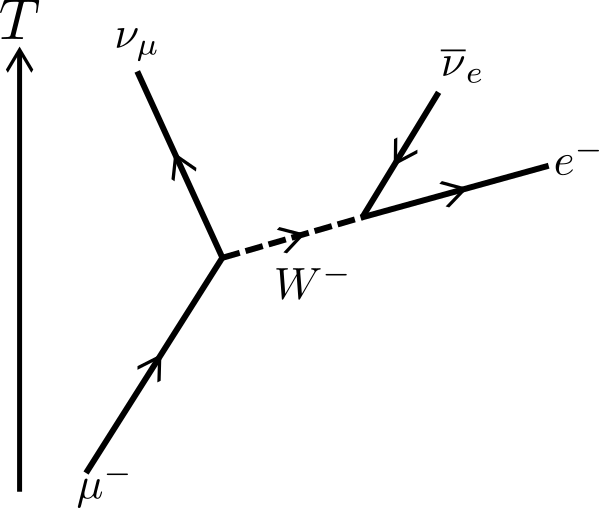
\includegraphics[width=0.4\textwidth]{Muon_Decay.pdf}
	\caption{Feynman-Diagramm des Zerfalls eines $\mu^-$}\label{img:zerfall}
\end{wrapfigure}
Durch die \tilt{primäre kosmische Strahlung} wird die Atmosphäre der Erde mit, größtenteils schweren Partikeln beschossen. Diese sind in der Regel Protonen und $\alpha$-Teilchen, können jedoch auch große Nuklide sein. Dieser Schauer aus schweren Teilchen wechselwirkt mit den Molekülen der Erdatmosphäre und zerfällt dabei, gegebenenfalls in mehreren Schritten, kaskadierend in seine Bestandteile. Das Zwischenprodukt der kosmischen Strahlung enthält, unter Anderem, Protonen, Pionen, Neutronen, Kaonen, Photonen, Elektronen und Positronen.\\
Das zu untersuchende Teilchen in diesem Versuch ist das Myon $\mu^\pm$, welches zusammen mit einem Anti-/Neutrino aus dem spontanen Zerfall eines Pions $\pi^\pm$ (Gl. (\ref{eq:plus}), (\ref{eq:minus})) entsteht.
\begin{align}
\pi^+\rightarrow&\mu^++\nu_\mu \label{eq:plus}\\
\pi^-\rightarrow&\mu^-+\overline{\nu}_\mu \label{eq:minus}
\end{align}
Die freien Myonen zerfallen nun mit hoher Wahrscheinlichkeit, unter Verlust ihrer kinetischen Energie, in ein Elektron/Positron und 2 jeweilige Anti-/Neutrinos.
\begin{align}
\mu^+\rightarrow& e^++\nu_e+\overline{\nu}_\mu\\
\mu^-\rightarrow& e^-+\nu_\mu+\overline{\nu}_e
\end{align}
\ref{img:zerfall} zeigt das Feynman-Diagramm des Zerfalls des Antimyons in ein Myonenneutrino, Elektronenantineutrino und Elektron. Dabei überträgt das negativ geladene Elementarteilchen des $W^-$-Bosons die elektroschwache Wechselwirkung, welche zur Erzeugung des Elektron-Antineutrino-Paares nötig ist.\\
Außerdem ist es möglich, dass der Myonen-Zerfall Photonen (Gl.(\ref{eq:phot})) aussendet, oder ein Elektron-Positron-Paar erzeugt (Gl. (\ref{eq:elekpos}).
\begin{align}
	\mu^-\rightarrow e^-+\overline{\nu}_e+\nu_\mu+\gamma \hspace{2cm} \mu^+\rightarrow e^++\nu_e+\overline{\nu}_\mu+\gamma \label{eq:phot}\\
	\mu^-\rightarrow 2e^-+e^++\overline{\nu}_e+\nu_\mu \hspace{2cm} \mu^+\rightarrow e^-+2e^++\nu_e+\overline{\nu}_\mu \label{eq:elekpos}
\end{align}
Mit sehr geringer Wahrscheinlichkeit kann ein negatives Myon mit einem Atom, unter Einfang eines Elektrons einer K-Schale, ein \tilt{myonisches Atom} bilden und dadurch in das Nuklid eingezogen werden. Die damit ausgelöste Umwandlung eines Protons in ein Neutron findet unter Emission eines $\nu_\mu$ statt. Experimentell bedeutet dies, das die real gemessene Zerfallszeit von Myonen größer ist als die des Vakuums.\\
Die Flussdichte der Myonen liegt bei etwa $\unit[100]{\frac{1}{m^2\cdot s}}$. Es gehört zu den Leptonen und ist einfach positiv bzw. negativ geladen (Anti-/Myon), wobei das Verhältnis $\mu^+/\mu^-=1,27$ beträgt. Es ist in seinen Eigenschaften vergleichbar mit dem Elektron: es besitzt einen Spin von $1/2$ und unterliegt nur der elektroschwachen, nicht jedoch der starken Wechselwirkung. Im Unterschied zum $e^-$ ist jedoch seine Masse um etwa das 200-fache größer und es besitzt nur eine mittlere Lebensdauer von $\unit[2,196\cdot 10^{-6}]{s}$. Der Fakt, dass wir trotzdem in der Lage sind, das Myon, welches in einer Höhe von rund $\unit[10]{km}$ in der oberen Atmosphäre entsteht, an der Erdoberfläche zu messen, ist Beweis für die relativistische Zeitdilatation bewegter Inertialsysteme.
\subsection{title}
\subsection{Myonenspektrometer}
\section{Durchführung}
\section{Auswertung}
\section{Quellen}
\end{document}